\chapter{Des solutions d'automatisation face à la masse des données}

Comme évoqué dans le chapitre précédent, l'augmentation exponentielle de la production documentaire impose la mise en place de solutions d'archivage capables de gérer efficacement cette masse croissante tout en maintenant un haut niveau de qualité dans le traitement des données. En effet, les fonds d'archives très volumineux posent un double défi : ils sont non seulement plus longs et complexes à décrire, mais leur manque de description approfondie peut les rendre inaccessibles. Sans une indexation efficace et des métadonnées descriptives interrogeables, ces fonds risquent de devenir inexploitables. Il est donc impératif de développer des stratégies pour maîtriser cette masse documentaire, notamment par l'élimination de fichiers quasi-identiques et par un signalement qui assure une indexation efficace. Ce chapitre propose d'explorer plusieurs solutions offertes par les technologies numériques pour automatiser le traitement archivistique dans ce contexte de production exponentielle. Nous commencerons par examiner les avantages et les inconvénients de l'intelligence artificielle, qui est devenue incontournable dans le paysage numérique actuel. Ensuite, nous nous pencherons sur des solutions moins coûteuses et plus accessibles, adaptées à des projets de petite à moyenne envergure. Enfin, nous aborderons les défis spécifiques liés à la volumétrie des reportages photographiques, en particulier dans le contexte des Archives nationales et du système d'archivage électronique Vitam, et les solutions sur mesure qui ont été adoptées pour surmonter ces obstacles.

\section{Avantages et inconvénients d’un recours à l’intelligence artificielle pour le traitement des archives iconographiques}

\subsection*{L'intérêt de l'intelligence artificielle pour l'indexation des archives iconographiques}

L’intelligence artificielle ouvre aujourd’hui la voie vers des solutions précieuses pour l’indexation des archives, notamment iconographiques, un domaine confronté à des défis liés à l’augmentation exponentielle de la production documentaire numérique. La capacité de l’IA à analyser et à traiter de grandes quantités d’images permet d'automatiser les processus d'indexation, rendant ainsi les archives plus accessibles et exploitables. Le \emph{deep learning}, une branche du \emph{machine learning}, est particulièrement pertinent dans ce contexte. Les algorithmes de \emph{deep learning}, inspirés par les réseaux de neurones du cerveau humain, sont capables de reconnaître des motifs complexes au sein des images\footcite[pp.3-4]{marcus2018deep}. Grâce à l'entraînement sur des ensembles de données volumineux et variés, ces algorithmes peuvent identifier et cataloguer les éléments visuels présents dans les photographies, comme des objets, des lieux, ou des personnes.

Le \emph{transfer learning}, qui permet d’adapter des modèles préexistants à de nouveaux ensembles de données sans ré-entraînement complet, confère une flexibilité supplémentaire à ces outils\footcite[pp.8-9]{marcus2018deep}. Cela signifie qu’une IA, entraînée initialement à reconnaître des motifs spécifiques, peut être réajustée pour répondre aux besoins d’un service d’archives, en se concentrant par exemple sur la reconnaissance de visages. Cette capacité d’analyse des images permet de générer automatiquement des mots-clés pertinents qui enrichissent les métadonnées associées aux fichiers, facilitant ainsi la recherche et l'interrogation des archives par les utilisateurs\footcite{langevinTechnologiesIntelligenceArtificielle2022}.

Si un algorithme est bien entraîné à reconnaître un humain, de nombreuses données d’entraînement demeurent nécessaires pour lui permettre de distinguer les individus et donc d’identifier précisément les personnes représentées : il faut lui avoir fourni en amont des données d’entraînement nombreuses sur chacune des personnes qu’on souhaite identifier. Un tel processus demande beaucoup de temps de préparation des données d’entraînement : il faut disposer de vues nombreuses et variées de toutes les personnes, lieux ou situations que l’on souhaite pouvoir identifier, et avoir procédé à cette indexation sur l’ensemble de ces données d’entraînement. De plus, ce travail de description nécessite en amont un autre travail de réflexion afin de déterminer les mots-clés que l’on souhaite faire remonter : comme nous l’évoquions au début de ce mémoire, le potentiel descriptif d’une photographie est presque illimité, il est donc difficile de déterminer au préalable l’ensemble des termes que l’on souhaite associer sans avoir dans un premier temps analysé le fonds dans son intégralité. Le \emph{clustering} permet une approche inverse qui ne repose pas sur une indexation préalable mais invite l’IA à proposer des regroupements de données en un nombre de catégories, prédéfini ou non, mais dont les critères de rassemblement sont déterminés par l’IA elle-même. Si cette solution semble plus adaptable, elle ne permet pas d’imposer un vocabulaire normé issu des réflexions des archivistes, et risque d’entraîner l’indexation de termes peu pertinents dans un contexte archivistique.

\subsection*{L'intérêt de l'IA pour identifier les photographies sensibles}

L’intelligence artificielle offre également de nouvelles possibilités dans la gestion des documents contenant des informations sensibles, qu'il s'agisse de données personnelles ou de contenus classifiés. L’enjeu est donc d’empêcher la communication de données sensibles, mais aussi de pouvoir librement communiquer les documents qui n’en contiendraient pas et dont les délais de communication sont repoussés en raison de l’incapacité des archivistes à analyser les fonds dans leur intégralité. Cette solution serait particulièrement intéressante dans le contexte des reportages photographiques de la Présidence dont le contenu potentiellement sensible impose le contrôle des fichiers demandés avant toute communication. 

L’IA peut jouer un rôle dans l’identification des photographies non communicables. Par exemple, les algorithmes de reconnaissance faciale peuvent être utilisés pour détecter et identifier les visages d'enfants, assurant ainsi le respect du droit à l'image des personnes mineures. De plus, elle peut être programmée pour analyser les titres ou les descriptions des reportages photographiques afin d’identifier des termes spécifiques, indiquant la présence de contenus sensibles protégés par le droit à l’image ou la législation sur la défense nationale. Dans ces cas, l’IA peut automatiquement assigner des règles de gestion spécifiques, telles que l’extension des délais de communicabilité ou l’obligation de flouter certaines parties des images avant leur diffusion\footcite{baronDarkArchivesEdemocracy2017}. Cette capacité à sécuriser et gérer automatiquement les archives sensibles non seulement protège les données mais assure également un meilleur respect des exigences légales et éthiques, tout en optimisant le processus de gestion documentaire.
Cependant, l'IA n'est pas infaillible et peut commettre des erreurs, notamment dans l'identification des visages ou l'attribution de mots-clés, ce qui peut avoir des conséquences significatives en matière de protection des données. Ainsi, un contrôle humain reste indispensable pour valider les résultats produits par les algorithmes et corriger les éventuelles anomalies.

\subsection*{Gérer la masse en identifiant les prises de vue quasi-identiques}
Il n’est pas question de procéder à des éliminations dans le contexte de la reprise des reportages photographiques aux Archives nationales. Les éliminations sont, le cas échéant, effectuées en amont par le service chargé de l’archivage intermédiaire. Cependant, d’un point de vue purement théorique, il peut être intéressant de s’interroger sur la pertinence de confier ce tri à une intelligence artificielle, les services versants n’ayant pas toujours les moyens de procéder à un tri efficace.

La gestion des prises de vue quasi-identiques, produites en rafale par des appareils numériques modernes, représente un défi majeur pour les archivistes chargés de fonds de photographies numériques. Ces séquences d'images, souvent très similaires, peuvent rapidement saturer les bases de données et rendre la gestion des archives plus complexe. L'intelligence artificielle offre une solution efficace à ce problème en identifiant et en regroupant ces images quasi-identiques. Grâce à des algorithmes spécialisés, l’IA peut analyser les variations minimes entre les prises de vue successives et les classer en groupes homogènes\footcite{rolan2019more}. Ce processus permet de réduire la redondance en sélectionnant automatiquement les images les plus représentatives de chaque séquence, tout en éliminant celles qui semblent redondantes. En conséquence, l'utilisation de l'IA permet d'alléger le volume des fichiers à traiter, de rationaliser l'organisation des archives et de faciliter l'accès aux documents les plus pertinents pour les utilisateurs. Cette gestion des images redondantes ne se limite pas à la réduction de la masse des archives, mais contribue également à l'optimisation des ressources de stockage.
La question subsiste toutefois des critères appliqués par l’algorithme pour sélectionner les clichés jugés les plus pertinents, une telle sélection pouvant être particulièrement subjective. Pour rendre un recours à l’IA adapté à ce contexte, il serait nécessaire d’ajouter une étape d’évaluation humaine des regroupements effectués.
\\

Malgré les promesses de l’IA dans le traitement des archives, il est essentiel de reconnaître les limites de ces technologies. Au-delà des limites évoquées précédemment, la mise au point et l’implémentation d’une IA dans un service nécessite des ressources humaines, financières et documentaires importantes pour le nettoyage et l’indexation des données d’entraînement, ainsi que pour garantir une puissance de calcul suffisante des machines locales. Par ailleurs, le jeu de données doit en valoir la chandelle : les données à traiter doivent être assez nombreuses pour que les données d’entraînement demeurent une minorité.

De plus, l'une des critiques majeures à l'encontre de l'IA concerne l'opacité de ses processus décisionnels, souvent qualifiés de \enquote{boîte noire}. L’absence de transparence dans le fonctionnement interne des algorithmes de \emph{deep learning} rend impossible la documentation des choix archivistiques, un aspect pourtant fondamental du métier d'archiviste. Cette opacité peut poser problème lorsqu’il s’agit de justifier les décisions prises par l’IA, notamment dans le cadre de l’évaluation et de la classification des documents. En conclusion, bien que l’IA offre des outils puissants pour améliorer le traitement des archives iconographiques, son intégration dans les pratiques archivistiques dépend des moyens du service, du délai de traitement permis, et de la volumétrie du fonds. Toutes ces limites excluent un recours à l’intelligence artificielle dans le contexte de la reprise des données des reportages photographiques de la Présidence de la République aux Archives nationales.

\section{Les possibilités actuelles de gestion de la masse aux Archives nationales}

Si une nouvelle évaluation ou un nouveau tri ne peuvent être réalisés, et que les moyens humains et le temps nécessaire pour décrire les photographies font défaut, le recours à l'intelligence artificielle devient également inenvisageable. Dans ce contexte, nous ne pouvons que nous tourner vers la solution initialement évoquée : exploiter les descriptions et indexations déjà produites par la cellule photographique. Il s'agit donc de tirer parti des ressources existantes, notamment en mettant en place des méthodes d'extraction en masse de ces métadonnées, en identifiant les doublons pour éviter l'archivage redondant, et en développant des solutions adaptées aux contraintes volumétriques imposées par le système d'archivage électronique Vitam.

\subsection*{Extraction et calcul de métadonnées en masse}

\subsubsection*{L'extraction de métadonnées techniques et descriptives avec Exiftool}

Il est relativement simple d'accéder aux métadonnées internes des images numériques. Certains visualiseurs d'images, comme XnView, permettent non seulement d'afficher le contenu graphique, mais également de consulter un large éventail de métadonnées associées aux fichiers. À défaut de disposer d'une application dédiée, un simple clic droit sur le fichier, suivi de l'option \emph{Propriétés}, ouvre une fenêtre où certaines métadonnées internes peuvent être consultées. Cependant, ces méthodes ne sont pas adaptées lorsque l'objectif est d'extraire en masse ces métadonnées et de sélectionner les plus pertinentes pour les intégrer à un processus de traitement des fichiers. Pour ce faire, des applications spécifiques dédiées à l'extraction des métadonnées internes sont nécessaires.

Au début de mon stage au DAD à l'été 2023, je me suis attachée à identifier une application répondant à ce besoin. Une analyse comparative avait déjà été réalisée dans le cadre du programme Vitam, répertoriant plusieurs logiciels d'extraction de métadonnées (tels qu'ExifTool, JHOVE, MediaInfo, File Investigator Engine, ImageMagick, et Apache Tika) et présentant les retours d'expérience d'institutions publiques les ayant testés dans le cadre de politiques de préservation numérique (notamment la BnF, Huma-Num, le Norwegian Research Council, et la National Library of Australia)\footcite[pp.19-42]{programmevitamExtractionMetadonneesTechniques2020}. À l'issue de cette analyse, ExifTool s'est distingué par son efficacité supérieure : il réussit à lire et à extraire les métadonnées de la plupart des fichiers, quel que soit leur type, et il se démarque par le nombre et la variété des métadonnées extraites. Par exemple, ExifTool parvient à extraire aussi bien des métadonnées techniques que descriptives, alors que d'autres outils, comme Metadata Extraction Tool, excellent dans l'extraction de métadonnées techniques, mais sont moins performants pour les métadonnées descriptives. En somme, ExifTool est l'outil qui extrait le plus grand nombre et la plus grande diversité de métadonnées, issues de formats variés. Convaincue par l'efficacité de cet outil, ainsi que par sa relative simplicité d'utilisation et son intégration potentielle dans une application future en Python, j'ai choisi de l'adopter.

Il s'agit d'un utilitaire open source en ligne de commande développé par Phil Harvey, qui permet de lire, écrire et éditer des métadonnées. Il prend en charge plusieurs types de métadonnées (EXIF, GPS, IPTC, XMP, JFIF, GeoTIFF, ICC Profile, Photoshop IRB, FlashPix, AFCP, ID3). L'outil est capable d'extraire l'ensemble ou une sélection de métadonnées sous forme de tableaux, de listes avec séparateurs point-virgule, ou encore sous des formats plus complexes comme XML/RDF ou JSON.

Voici par exemple à quoi peut ressembler une commande Exiftool exécutée dans une invite de commande : 

\begin{displayquote}
	\begin{center}
\textbf{exiftool -csv -r -filename -artist -createdate -title -city -country -keywords -charset utf8 . }
\end{center}
\end{displayquote}

\begin{itemize}
	\item La mention d'\enquote{exiftool} en début de commande indique à l'ordinateur l'application qu'il doit exécuter.
	\item \enquote{-csv} indique la forme sous laquelle on souhaite obtenir l'extraction de métadonnées. Ici, la commande permet d'obtenir un fichier CSV, donc sous une forme tabulaire. Si l'on souhaitait obtenir les mêmes informations au format JSON par exemple, il suffirait de remplacer cette commande par \enquote{-json}.
	\item \enquote{-r} commande à l'application d’analyser les fichiers contenus dans les sous-répertoires du dossier cible.
	\item Les commandes suivantes correspondent simplement aux noms des métadonnées à extraire. Pour les connaître, il faut se référer aux descriptions des schémas de métadonnées (XMP, EXIF, IPTC).
	\item \enquote{-charset utf8} indique l'encodage dans lequel on souhaite que les métadonnées soient exportées. Cette fonction est particulièrement utile face à des fonds anciens ou produits sur des appareils Apple, souvent encodés en Latin1 plutôt qu'en UTF-8.
	\item Le point en fin de commande indique que l'application doit analyser l’ensemble des fichiers du répertoire dans lequel l’invite de commande a été ouverte. Pour analyser un répertoire spécifique, il faut remplacer le point par le chemin du répertoire entre guillemets.
\end{itemize}


\subsubsection*{Identification de formats et calculs d'empreintes avec DROID et Siegfried}

Pour l'analyse des formats, j'ai utilisé les logiciels les plus couramment employés par le DAD, à savoir DROID\footcite{droid2024} et Siegfried\footcite{itforarchivists2024}.

DROID et Siegfried sont des logiciels libres et open source conçus pour l'identification automatisée des formats de fichiers. Ces outils s'appuient sur la reconnaissance des signatures internes des fichiers et intègrent les informations du registre technique \gls{pronom} des Archives nationales du Royaume-Uni.

DROID offre l'avantage d'une interface utilisateur qui permet de sélectionner les informations à exporter. De plus, l'export peut se faire sous forme tabulaire, ce qui facilite la lecture et la compréhension par un utilisateur humain. Dans le cadre de la reprise des reportages photographiques, j'ai utilisé DROID pour identifier les formats présents dans les fonds, ce qui m'a permis de repérer les plus courants ainsi que les plus inattendus (tels que des PDF, des documents Microsoft Word ou des vidéos), enrichissant ainsi notre compréhension du fonds. Cette identification a également permis de détecter les fichiers au format propriétaire, les fichiers système, ou encore les fichiers RAW, que nous avons choisi d'exclure de la reprise des données. Les formats propriétaires, en effet, sont plus difficiles à pérenniser, nécessitant souvent des logiciels payants pour être ouverts et présentant ici un intérêt limité (comme les fichiers Photoshop sans modifications significatives ou avec un équivalent en JPEG). DROID permet aussi d'identifier les fichiers endommagés, tels que des fichiers avec l'extension JPEG dont la signature n'a pas pu être identifiée. Si ces fichiers endommagés étaient toujours lisibles, ils ont été conservés; dans le cas contraire, ils ont été supprimés.

Bien que DROID soit très utile pour l'analyse des fonds, il est moins adapté à une intégration fluide dans un pipeline de traitement de données. Pour l'extraction et l'exploitation des informations, nous avons donc opté pour Siegfried. Cet outil est très simple d'utilisation en ligne de commande : il suffit d'exécuter la commande \enquote{sf FILE} pour identifier les informations de format d'un fichier (où FILE correspond au chemin du fichier) ou \enquote{sf DIR} pour analyser tous les fichiers d'un répertoire (où DIR correspond au chemin du répertoire). À l'instar d'Exiftool, Siegfried permet également de choisir le format des données générées.

Voici un exemple d'utilisation de Siegfried en ligne de commande : 

\begin{displayquote}
	\begin{center}
		\textbf{sf -hash sha512 -json "/home/port-pret-etu01/Images/image.jpg"}
	\end{center}
\end{displayquote}

\begin{itemize}
	\item \enquote{sf} indique à l'ordinateur qu'il doit utiliser l'application Siegfried.
	\item \enquote{-hash sha512} commande à Siegfried de calculer l'empreinte des fichiers analysés en utilisant l'algorithme appelé sha512.
	\item \enquote{-json} indique à Siegfried le format attendu pour la restitution des métadonnées calculées.
	\item La dernières information entre guillemets correspond au chemin du fichier ou du répertoire à analyser.
\end{itemize}


\subsection*{Les méthodes d’identification des doublons}

Comme mentionné précédemment, l'analyse des empreintes de fichiers permet d'identifier les doublons \enquote{techniques}, c'est-à-dire des fichiers d'un même format contenant exactement le même contenu informationnel et les mêmes métadonnées internes. Cependant, nous avons rencontré une situation où cette méthode s'est avérée insuffisante pour détecter des prises de vue identiques.

Le versement des reportages photographiques de la présidence de Jacques Chirac est réparti en trois dossiers : les reportages traités, les reportages non traités, et un ensemble de neuf reportages découverts sur des CD en 2019 lors d'un chantier de reconditionnement des photographies argentiques. Les reportages retrouvés sur CD existant également sur serveur, nous avons cherché à identifier les doublons entre ces deux supports. Grâce à un export des métadonnées internes réalisé avec Exiftool, nous avons pu confirmer que les métadonnées descriptives n'étaient pas renseignées dans les reportages sur CD. Il s'agissait donc probablement d'une version des fichiers antérieure à leur traitement et à leur description dans une photothèque. Cependant, le calcul des empreintes par DROID ne permet pas d'identifier des photos identiques dont les métadonnées internes diffèrent. En revanche, le logiciel ImageMagick\footnote{Voir le site de présentation et de téléchargement du logiciel ImageMagick : \url{https://imagemagick.org/index.php}.} calcule l'empreinte en se basant uniquement sur les pixels, répondant ainsi parfaitement à notre besoin. Il convient toutefois de souligner les limites de cette fonctionnalité : le calcul des empreintes de deux images identiques peut différer si elles n'ont pas le même format, et la méthode de calcul varie d'une version du logiciel à l'autre, ce qui signifie que l'empreinte d'un même fichier peut être différente selon la version utilisée. Si ces limites ne posaient pas de problème dans notre travail, elles doivent être prises en compte pour une utilisation plus généralisée d'ImageMagick. Les variations des empreintes d'un même fichier selon les versions rendent ce logiciel peu adapté pour garantir l'intégrité d'un fichier image sur le long terme.

\section{La volumétrie : un obstacle insurmontable aux Archives nationales ?}

La volumétrie importante des fonds de reportages photographiques pose non seulement un problème d'appréhension et de description, mais aussi un problème de manipulation. En effet, plus la masse de données à déplacer est importante, plus les contraintes s'accumulent : le déplacement prend plus de temps, ce qui augmente la probabilité d'un problème technique interrompant le processus, risquant non seulement d'endommager les fichiers mais de perdre ceux n'ayant pas pu être déplacés, et les applications métier peuvent ne pas être capables de manipuler de telles quantités de données. C'est pas exemple le cas du module des entrées unitaires du SAE des Archives nationales. 

\subsection*{Les contraintes volumétriques des entrées unitaires dans le SAE des Archives nationales}

L'un des principaux défis à l'automatisation du traitement et du versement des reportages photographiques réside dans les restrictions de volumétrie imposées par le système d'archivage électronique des Archives nationales. En effet, pour les versements sous forme d'entrées unitaires, les paquets ne doivent pas excéder 30 Go. Cette contrainte constitue non seulement un obstacle pour le versement des reportages photographiques, mais peut également rendre certains versements impossibles, en particulier ceux relatifs à des fichiers audiovisuels d'images animées dont le volume unitaire dépasse largement les 30 Go.

Pour rappel, les reportages de la mandature de François Hollande représentent un volume de 2,6 To, ceux de la mandature de Nicolas Sarkozy un volume de 1,3 To, et ceux de la mandature de Jacques Chirac plus de 600 Go. Ainsi, il faudrait plus de 88 paquets pour verser les reportages de François Hollande, plus de 45 pour ceux de Nicolas Sarkozy, et plus de 20 pour ceux de Jacques Chirac, soit un total de plus de 154 paquets. Durant mon stage de deuxième année, entre avril et juillet 2024, l'origine de cette limitation a pu être identifiée. Elle pourra donc être corrigée, ce qui permettra d'augmenter la taille des paquets à verser. Bien que cette limitation ne puisse jamais être totalement supprimée, elle pourrait être relevée à 100 Go, ce qui réduirait considérablement le nombre de paquets nécessaires.

Les scénarios de versement envisagés pour chaque entrée ont donc dû intégrer cette contrainte volumétrique en divisant l'entrée en plusieurs versements. Pour chaque entrée, un premier SIP appelé \enquote{SIP chapeau} ne contient pas de données, mais établit l'architecture de l'entrée telle qu'elle devra apparaître dans le SAE Vitam : une unité archivistique racine représentant l'entrée dans son ensemble, par exemple \enquote{Reportages photographiques de la mandature de François Hollande}, suivie d'une unité archivistique de niveau \enquote{dossier} pour chaque année de la mandature. Les SIP suivants, chacun contenant un ensemble de reportages plus ou moins important, permettront de restituer l'arborescence de ces reportages sous l'unité archivistique de l'année correspondante.

\subsection*{Définition d'une méthode d'ajustement manuel de la taille des paquets d'archives}

Cette contrainte volumétrique a conduit à une réflexion approfondie sur la méthode la plus efficace pour contrôler la taille des paquets. Dans un premier temps, nous avions envisagé de développer une application capable de constituer un SIP à partir du contenu d’un répertoire. Cependant, cette approche nécessitait de copier l’ensemble des reportages traités avant de préparer chaque paquet, ce qui augmentait considérablement les risques de perte de données et l’espace de stockage requis sur les machines utilisées.

Il est donc apparu plus pertinent d'intégrer directement à l'application une méthode de limitation de la taille des SIP. Une première approche envisageait de se baser sur la taille prévue du paquet : l’application récupérerait les reportages dans l’ordre de leur apparition dans le répertoire de stockage, tout en respectant une limite volumétrique prédéfinie. Cette méthode avait l’avantage de s’adapter aux éventuelles évolutions du système d'archivage électronique des Archives nationales. Cependant, elle présentait deux inconvénients : elle laissait l'application définir l'ordre des reportages à inclure, suivant simplement l’ordre des dossiers. Ainsi, en cas de variations dans le nommage des dossiers, l’ordre suivi par l’application risquait de ne pas correspondre à l’ordre intellectuel des reportages. De plus, selon le contexte d’utilisation, l'archiviste pouvait souhaiter une division plus sémantique, par exemple en fonction de critères temporels plus fins (par mois, par exemple), ce que cette méthode ne permettait pas.

Nous avons donc opté pour une sélection manuelle des reportages à intégrer dans chaque paquet, en utilisant comme référence un élément clé : le numéro de reportage, présent à la fois dans l'instrument de recherche et dans le nommage des dossiers. Les numéros des reportages à inclure sont saisis dans un fichier texte, que l'application utilise pour les identifier dans le répertoire de stockage. Bien que plus manuelle, cette méthode permet à l’archiviste un meilleur contrôle de la composition des paquets.


\subsection*{Face à la nécessité d'un versement en plusieurs paquets : envisager les méthodes de classement}

Les versements devront ensuite être regroupés au sein du système d'archivage électronique (SAE) pour reconstituer l'arborescence originale des dossiers et sous-dossiers. Le SAE Vitam propose trois méthodes de rattachement, parmi lesquelles deux ont été employées pour la reprise des données des reportages photographiques des services du Premier ministre et de la Présidence de la République.

La première méthode, appelée \enquote{reclassement}, est directement accessible via l'interface du SAE des Archives nationales. Après le versement de plusieurs paquets, effectué dans un ordre précis, il est nécessaire d’indiquer le niveau auquel chaque paquet doit être placé par rapport au SIP chapeau représentant l’arborescence. Les données de chaque SIP sont alors déplacées à leur place dans l'arborescence. Cette méthode, choisie pour le versement des reportages photographiques des services du Premier ministre, est relativement simple mais comporte deux risques, non évalués mais ne pouvant être exclus : un risque d'erreur entraînant une perte lors du déplacement des fichiers, et un risque d'erreur humaine dans l’ordre des paquets versés et reclassés.

Pour les reportages photographiques de la Présidence de la République, nous avons opté pour la seconde méthode. Celle-ci consiste à indiquer dans le manifest du SIP sous quelle unité d'archive l'ensemble du paquet doit être placé dans le SAE. Cette unité parente est spécifiée par sa cote. Une unité archivistique \enquote{fantôme} est ajoutée au SIP à rattacher pour représenter l’unité parente de tous les reportages du paquet. Des métadonnées de gestion associées à cette unité \enquote{fantôme} indiquent qu’elle correspond à l’unité archivistique déjà versée à laquelle le paquet devra être rattaché. Cette méthode ne passe pas l'interface du SAE, contrairement à la première, elle nécessitent donc d'être implémenter au cours de l'étape de création des paquets.

Voici une modélisation de la structure d'un versement utilisant cette méthode de rattachement :

\begin{figure}[h]
	\begin{adjustbox}{width = \textwidth, center}
		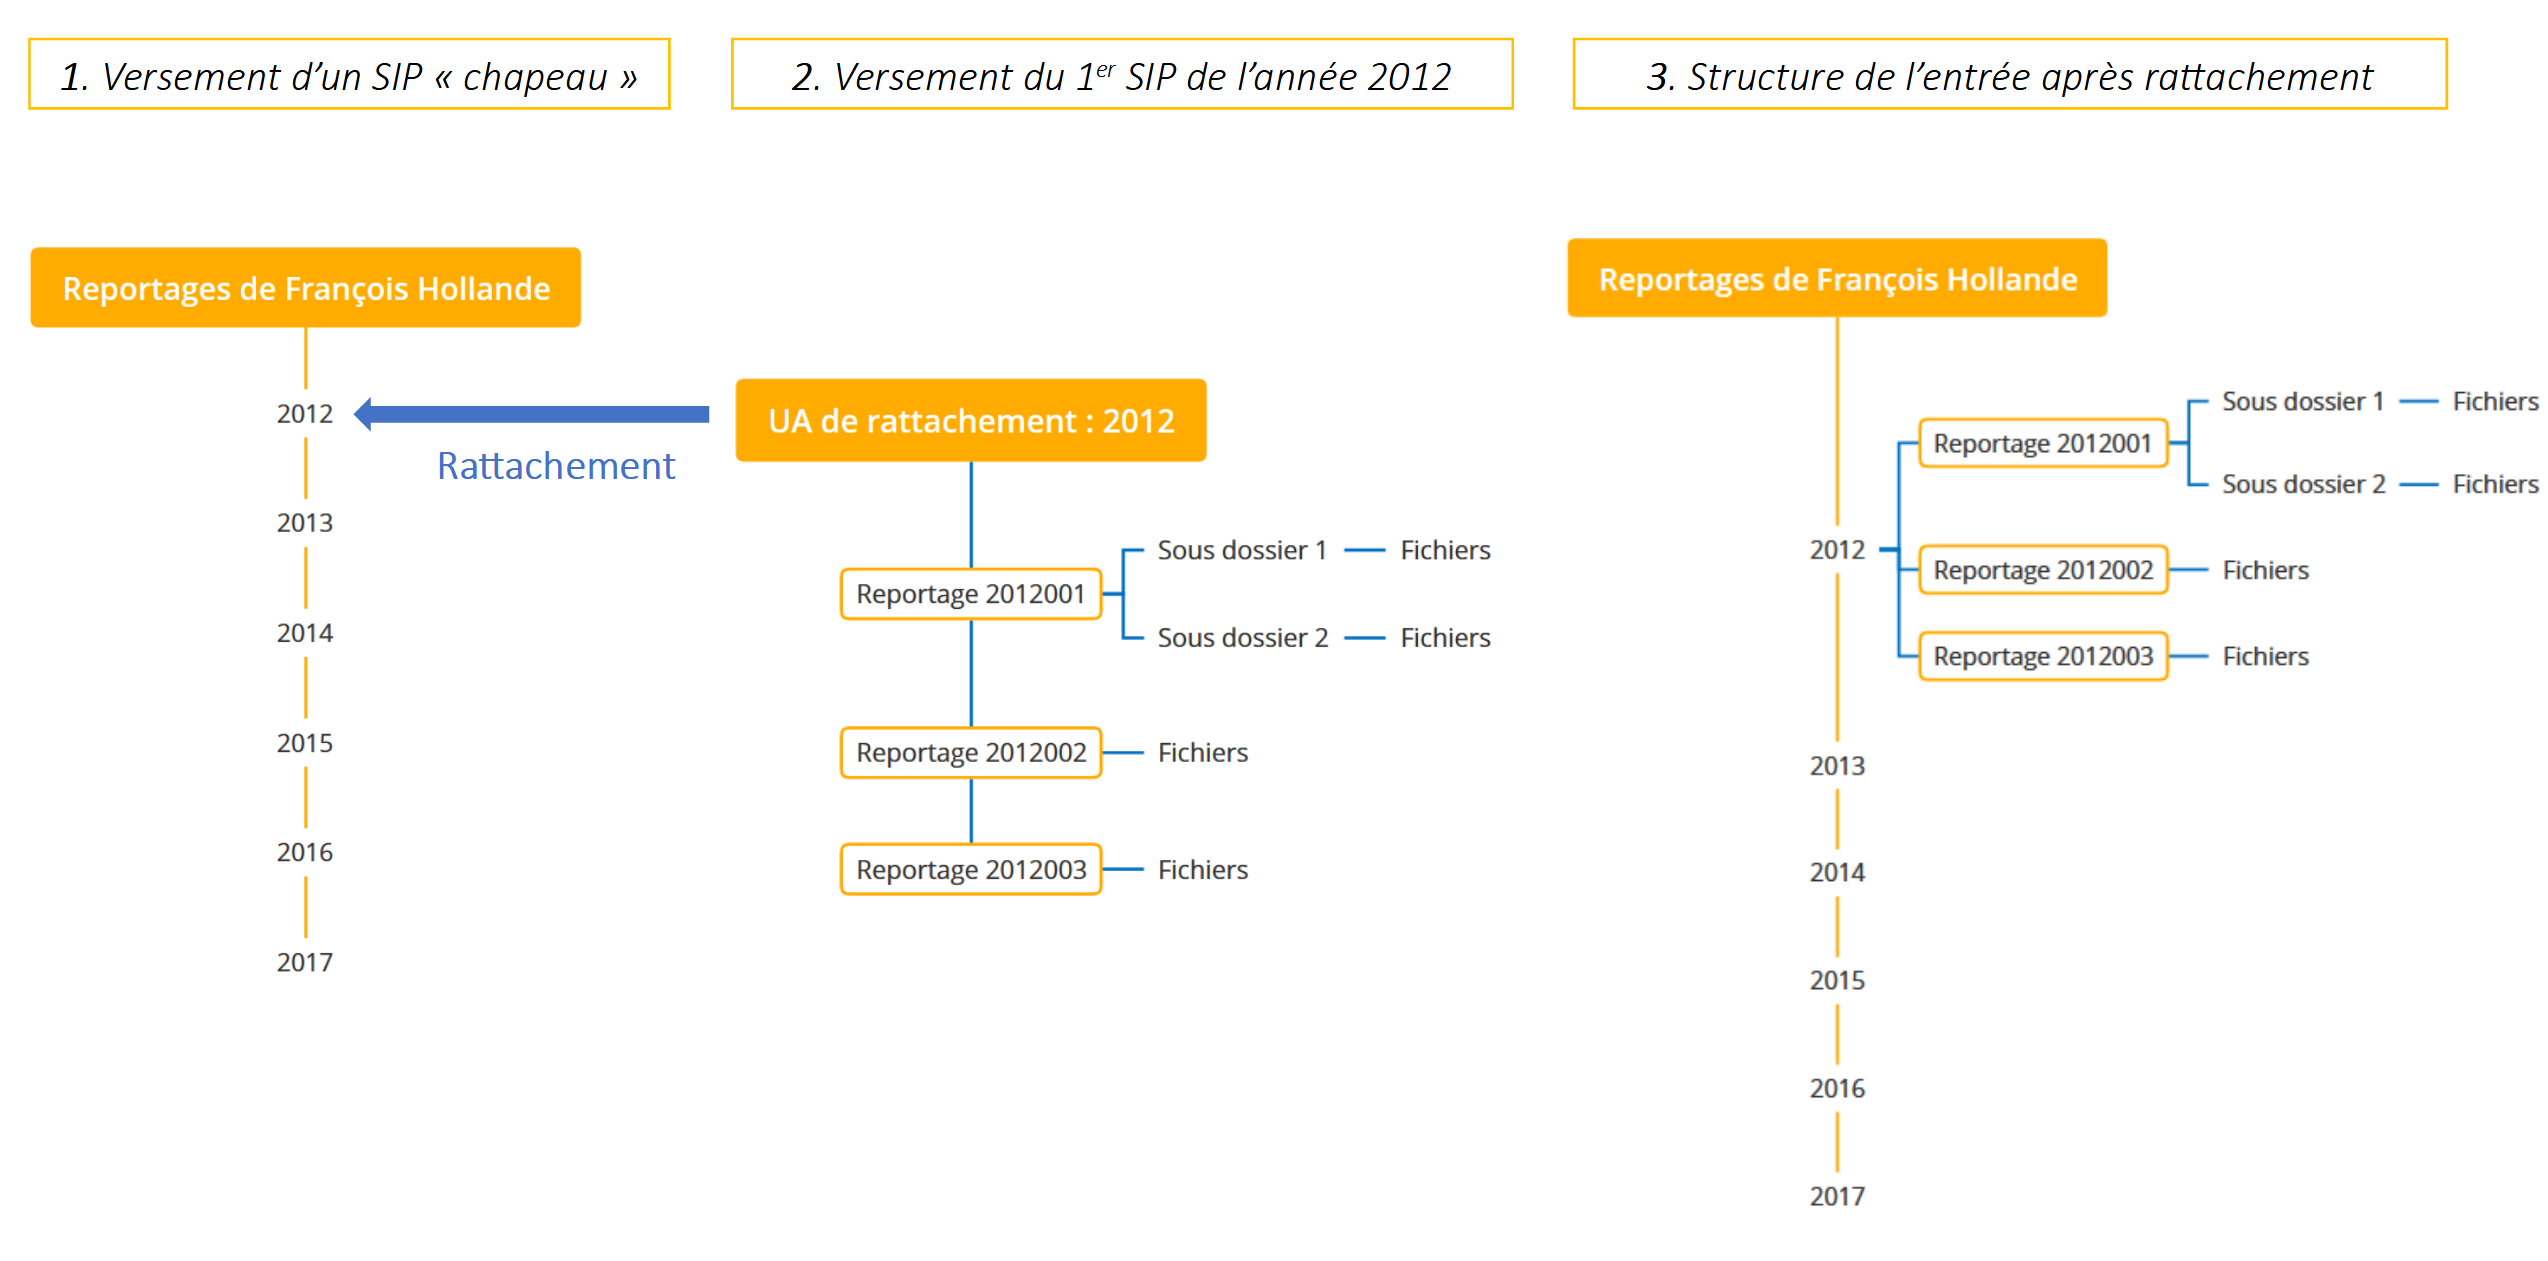
\includegraphics{./img/schema_rattachement.png}
	\end{adjustbox}
	\caption{Modélisation du processus de rattachement choisi pour les versements des reportages de la Présidence de la République.}
\end{figure}

Dans le cadre de la reprise des reportages photographiques, il était essentiel de comprendre non seulement le contexte institutionnel et technique de production des fichiers, mais aussi leur évolution depuis leur création jusqu'à leur reprise actuelle. En analysant l'impact de ce contexte de production sur la qualité des métadonnées descriptives, nous avons pu mettre en lumière tant les intérêts que les limites de leur utilisation dans un cadre archivistique. L'exemple de la collecte de reportages photographiques par la Bibliothèque nationale de France témoigne du fait que les défis rencontrés aux Archives nationales sont partagés par toutes des institutions patrimoniales confrontées à cette typologie documentaire.

Pour appréhender les exigences techniques auxquelles notre application devait répondre, il était indispensable de présenter l'environnement normatif et institutionnel de l'archivage électronique, ainsi que les traitements antérieurs appliqués dans le cadre des méthodes d'archivage précédentes. Les modifications introduites par le programme Constance ont, en effet, un impact direct sur la reprise des données, qui se décline en deux principales méthodes selon qu'il s'agisse de reportages traités ou non traités. Enfin, notre travail s'inscrit dans la méthodologie définie par le Département de l'administration des données pour l'ensemble du chantier de reprise des données. Cette méthodologie a été décrite, tout comme les contraintes spécifiques rencontrées dans le contexte très particulier de l'archivage électronique au sein du SAE Vitam des Archives nationales.

Tout ce travail de compréhension du contexte institutionnel et technique, de recherche des possibilités offertes par les technologies numériques, ainsi que la réflexion sur les enjeux archivistiques liés à la reprise de ce fonds, avait pour objectif de concevoir une méthode d'automatisation du traitement de ces reportages photographiques, garantissant ainsi leur accessibilité future. Dans la prochaine partie de ce mémoire, nous présenterons les réalisations concrètes effectuées au cours de ce stage, en particulier le pipeline de données, qui incarne l'aboutissement de cette méthode et sa mise en \oe{}uvre.